\documentclass[tikz,border=6pt]{standalone}
\usepackage{amsmath}
\usetikzlibrary{arrows.meta,calc}
\begin{document}
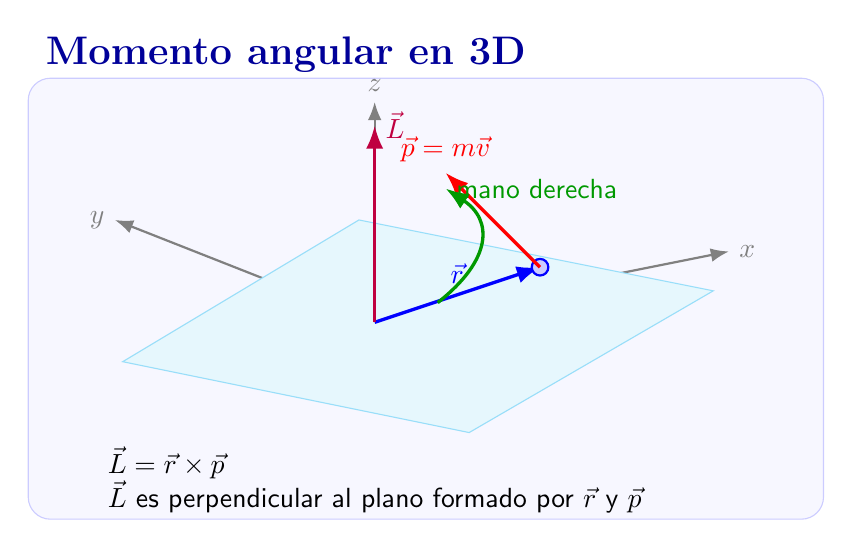
\begin{tikzpicture}[>=Latex, font=\sffamily]
  \node[anchor=west, text=blue!60!black, font=\bfseries\Large] at (-4.3,3.4) {Momento angular en 3D};
  \draw[rounded corners=8pt, fill=blue!3, draw=blue!20] (-4.4,-2.5) rectangle (5.7,3.1);
  \coordinate (O) at (0,0);
  \draw[->, gray, thick] (O) -- (4.5,0.9) node[right] {$x$};
  \draw[->, gray, thick] (O) -- (-3.3,1.3) node[left] {$y$};
  \draw[->, gray, thick] (O) -- (0,2.8) node[above] {$z$};
  \filldraw[fill=cyan!10, draw=cyan!40] (-3.2,-0.5) -- (1.2,-1.4) -- (4.3,0.4) -- (-0.2,1.3) -- cycle;
  \coordinate (R) at (2.1,0.7);
  \draw[->, very thick, blue] (O) -- (R) node[midway, above] {$\vec r$};
  \fill[blue!20, draw=blue, thick] (R) circle (3pt);
  \draw[->, very thick, red] (R) -- ++(-1.2,1.2) node[above] {$\vec p=m\vec v$};
  \draw[->, very thick, purple] (O) -- (0,2.5) node[right] {$\vec L$};
  \draw[->, very thick, green!60!black] (0.8,0.25) .. controls (1.5,0.8) and (1.5,1.3) .. (0.9,1.7) node[right] {mano derecha};
  \node[align=left] at (0,-2.0) {$\vec L=\vec r\times\vec p$\\$\vec L$ es perpendicular al plano formado por $\vec r$ y $\vec p$};
\end{tikzpicture}
\end{document}
